\documentclass[tikz,border=9pt]{standalone}
\usepackage{amsmath}
\usetikzlibrary{arrows.meta,fit}
\begin{document}
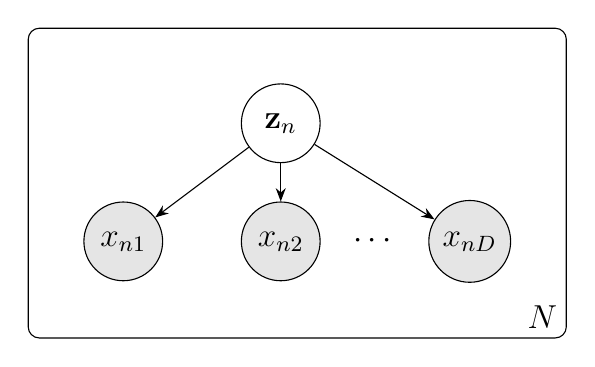
\begin{tikzpicture}[>=Stealth,latent/.style={circle,draw,minimum size=10mm},obs/.style={latent,fill=gray!20},font=\large]
\node[latent] (z) at (0,1.5) {$\mathbf z_n$};
\node[obs] (x1) at (-2,0) {$x_{n1}$};
\node[obs] (x2) at (0,0) {$x_{n2}$};
\node (dots) at (1.2,0) {$\cdots$};
\node[obs] (xd) at (2.4,0) {$x_{nD}$};
\foreach \v in {x1,x2,xd}{\draw[->] (z)--(\v);}
\node[draw,rounded corners,fit=(z)(x1)(x2)(xd),inner sep=7mm] (plate) {};
\node[anchor=south east] at (plate.south east) {$N$};
\end{tikzpicture}
\end{document}
